\documentclass[10pt,twocolumn]{article}
\usepackage[margin=0.72in,columnsep=0.26in]{geometry}
\usepackage{amsmath,amssymb}
\usepackage{graphicx}
\usepackage{xcolor}
\usepackage{array}
\usepackage[hidelinks]{hyperref}

\definecolor{accent}{RGB}{30,58,138}
\renewcommand{\arraystretch}{1.15}

\title{\Large\bfseries Conquering \textit{Samurai Shodown II} on a Single Machine:\\
A Hardware-Grounded Mixture-of-Experts Architecture with Physical-Invariant Best-of-3 Arbitration}

\author{Samurai Shodown II AI Project (\texttt{footballqq})\\
\small Open-Source Release: \url{https://github.com/footballqq/samsho2-moe-ai}}
\date{November 2026}

\begin{document}
\maketitle

\begin{abstract}
Training autonomous fighting-game agents on classic arcade hardware under single-machine compute budgets presents compounding challenges: extreme damage lethality, severe inter-character gradient conflict, camera-zoom HUD distortion, and subtle evaluation pitfalls across multi-round Best-of-3 (Bo3) matches. In this system and empirical methodology paper, we document the end-to-end engineering of an autonomous AI agent for SNK's Neo-Geo weapon fighter \textit{Samurai Shodown II} (\texttt{samsho2}) running on MAME 0.281. Rather than relying on monolithic from-scratch reinforcement learning—which empirically collapsed into passive corner-turtling and cross-opponent forgetting on a single PC—we introduce a four-layer architecture combining: (1) direct Neo-Geo WRAM hardware entity perception (\texttt{UID+0xBB} authoritative health, normalized distance, hit-damage latch, and hardware-verified character IDs \texttt{0x00}--\texttt{0x10}); (2) a 9-action Semi-Markov Decision Process (SMDP) semantic combat intent space; (3) a physically isolated Mixture-of-Experts (MoE) router pairing per-round policies with closed-loop distance-reactive controllers (\texttt{DistanceReactivePolicy}); and (4) a physical-invariant Bo3 match arbiter (\texttt{Bo3MatchController}) designed in response to two real evaluation failures (BUG-17 timeout sign inversion and BUG-18 phantom-round flicker). Across live 60~FPS MAME emulation, AI Haohmaru achieves 16/16 full-roster Bo3 victories—verified with 18.0-second post-KO celebration recordings and bilingual commentary timelines—and supports zero-conflict True 2P VS human-versus-AI play. We candidly analyze the generalization limits of sequence-heavy experts against adaptive human tactics and outline a concrete MoE-to-PPO and Offline RL roadmap.
\end{abstract}

\noindent\textbf{Index Terms}---Fighting Game AI, Mixture of Experts, Semi-Markov Decision Process, Arcade Emulation, Evaluation Integrity, Reinforcement Learning.

\section{Introduction}
Classic 2D arcade fighting games have long served as demanding testbeds for sequential decision-making because they combine tight 60~Hz reaction windows, asymmetric character mechanics, and non-transitive rock-paper-scissors combat dynamics~\cite{lu2013fightingice,vinyals2019alphastar}. Among classic fighters, SNK's 1994 Neo-Geo masterpiece \textit{Samurai Shodown II} (\texttt{samsho2}) introduces particularly unforgiving weapon-based mechanics: a single heavy slash can remove 30\%--50\% of a fighter's health, camera zoom dynamically rescales the viewport as fighters separate, and Best-of-3 (Bo3) matches feature \emph{asymmetric round refill} where the round loser refills to full stamina while the round winner retains leftover health.

In early single-machine experiments using standard Proximal Policy Optimization (PPO)~\cite{schulman2017ppo}, we encountered three recurring failure modes: (i) a \emph{passive turtle trap} where whiff and damage penalties made retreating to the corner yield higher expected return than attacking; (ii) \emph{inter-character gradient conflict}, where opposing counters required across 16 diverse opponents overwrote shared network weights; and (iii) \emph{simulator throughput constraints} on consumer CPU hardware. Furthermore, two severe evaluation bugs—an inverted time-over arbiter (BUG-17) and transition-flicker phantom rounds (BUG-18)—demonstrated that unverified automated metrics can fabricate artificial win-rate improvements.

Positioned as an empirical system and engineering lessons-learned paper, this work makes four practical contributions:
\begin{enumerate}
    \item \textbf{Hardware-Grounded WRAM Perception \& SMDP Abstraction}: We expose authoritative Neo-Geo WRAM entity fields through a lockstep MAME 0.281 Lua TCP bridge and compress raw frame-level inputs into 9 semantic combat intents.
    \item \textbf{Decoupled MoE with Closed-Loop Reactive Experts}: We isolate all 16 opponents into independent JSON expert policies, introducing a closed-loop \texttt{DistanceReactivePolicy} that solves fullscreen boss zoning (\textit{Mizuki} and \textit{Sieger}) where open-loop sequences fail.
    \item \textbf{Physical-Invariant Bo3 Arbitration}: We formalize six evaluation integrity rules and a three-guard \texttt{Bo3MatchController} that eliminates timeout sign bugs and phantom-round miscounts.
    \item \textbf{Full 16/16 Verification, True 2P VS Mode, and Open Release}: We verify all 16 matchups via 60~FPS MP4 recordings with 18.0~s post-match settlement holds, deliver zero-conflict 2P VS human-versus-AI play, and release a clean, self-contained repository.
\end{enumerate}

\section{Related Work}
\textbf{Fighting Game AI and Emulation Testbeds.} Research in fighting-game AI has spanned rule-based and Monte Carlo Tree Search agents in FightingICE~\cite{lu2013fightingice}, deep RL on \textit{Street Fighter II/III} via Gym-Retro and MAME bridges, and large-scale self-play leagues~\cite{vinyals2019alphastar}. Unlike custom research simulators that expose clean JSON APIs, emulating authentic Neo-Geo arcade ROMs in MAME requires reverse-engineering Work RAM (WRAM) memory layouts and handling non-deterministic arcade scene transitions.

\textbf{SMDP Macro Actions and Mixture of Experts.} Temporal abstraction via options and Semi-Markov Decision Processes (SMDPs)~\cite{sutton1999options} dramatically reduces effective horizon length in high-frequency control. Mixture-of-Experts architectures~\cite{jacobs1991moe} mitigate negative transfer by partitioning distinct regimes across specialized modules. In our setting, static opponent-ID routing over isolated expert policies guarantees zero cross-character regression.

\textbf{Evaluation Integrity and Offline RL.} Specification gaming and evaluator bugs are well-documented hazards in RL~\cite{amodei2016concrete}. Our BUG-17 and BUG-18 postmortems echo the need for independent physical invariants and human visual gating. Looking forward, Behavior Cloning, Kickstarting~\cite{schmitt2018kickstarting}, Go-Explore~\cite{ecoffet2021goexplore}, and Implicit Q-Learning (IQL)~\cite{kostrikov2022iql} offer principled paths to distill our MoE assets into generalizable neural policies.

\begin{figure*}[t]
    \centering
    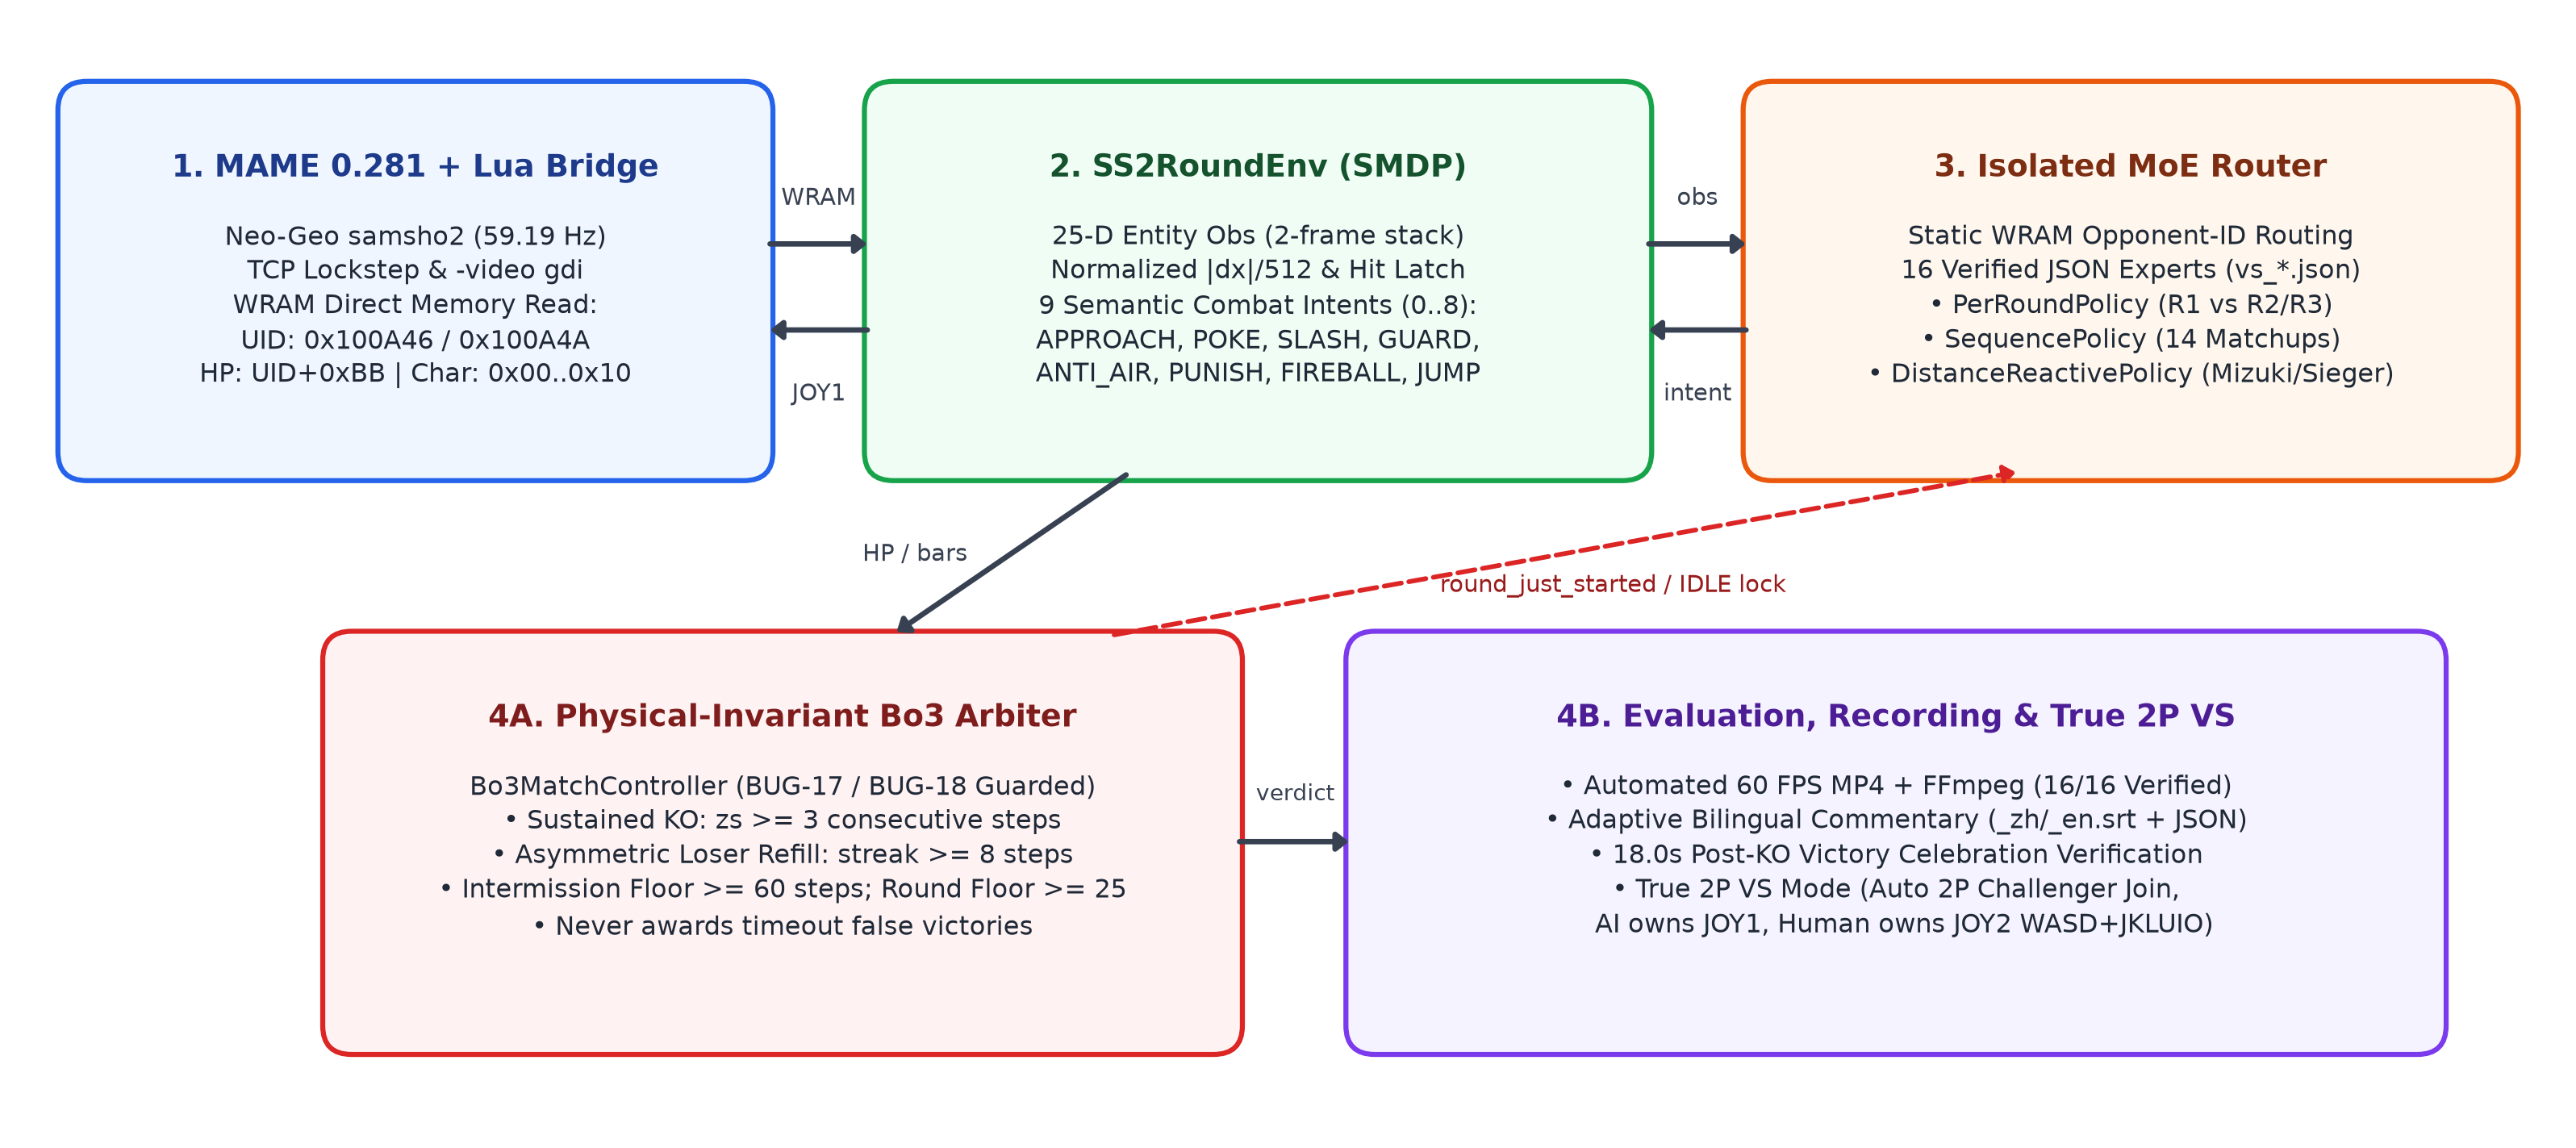
\includegraphics[width=0.96\textwidth]{figures/fig1_architecture.png}
    \caption{Four-layer architecture of the \textit{Samurai Shodown II} MoE system: (1) MAME 0.281 Lua TCP bridge with direct WRAM reading; (2) \texttt{SS2RoundEnv} SMDP environment exposing 25-D entity observations and 9 semantic intents; (3) physically isolated MoE router combining per-round sequence and closed-loop distance-reactive policies; and (4) physical-invariant Bo3 arbitration driving 60~FPS multimodal recording and True 2P VS human play.}
    \label{fig:arch}
\end{figure*}

\section{System Architecture \& Hardware Perception}
Figure~\ref{fig:arch} summarizes our four-layer system architecture.

\subsection{MAME 0.281 Lockstep Bridge \& Reliability}
Our Lua bridge (\texttt{mame/bridge.lua}) communicates over a dynamically bound localhost TCP socket. To guarantee unattended stability during batch recording on Windows, MAME runs with software GDI rendering (\texttt{-video gdi}) rather than Direct3D, preventing GPU Timeout Detection and Recovery (TDR) crashes during screen lock. Every bridge session runs under a Win32 Job Object (\texttt{win32\_process.py}) so orphaned emulator processes are automatically reaped on termination.

\subsection{Direct Neo-Geo WRAM Entity Perception}
Pixel-based health bar parsing in \textit{Samurai Shodown II} suffers from three failure modes: camera zoom-out distortion, rage-flash palette shifts, and 15--30 frame animation lag. We instead read authoritative entity memory directly:
\begin{itemize}
    \item \textbf{Dynamic Entity Pointers}: P1 and P2 entity base addresses (\texttt{UID}) reside at \texttt{0x100A46} and \texttt{0x100A4A}.
    \item \textbf{Authoritative Logical Health}: \texttt{UID + 0xBB} stores 1-byte unsigned health (base maxima: 128 standard, 164 for Ukyo, 186 for Sieger).
    \item \textbf{Hit-Damage Latch}: \texttt{0x105ED3} latches immediately upon hit connection, enabling lag-free whiff verification.
    \item \textbf{Hardware Character IDs (\texttt{UID + E\_CHAR})}: Live probing across all 16 savestate anchors revealed that slot \texttt{0x0A} is reserved (Kuroko), shifting Charlotte through Mizuki to \texttt{0x0B}--\texttt{0x10} (\texttt{0x0B}: Charlotte, \texttt{0x0C}: Genjuro, \texttt{0x0D}: Cham Cham, \texttt{0x0E}: Sieger, \texttt{0x0F}: Nicotine, \texttt{0x10}: Mizuki). Correcting this hardware table eliminated misrouting in live 2P VS character detection.
\end{itemize}

Each step produces a 25-dimensional entity observation stacked over 2 consecutive steps (50-D), including signed horizontal offset, normalized distance $|dx|/512$ (channel~1), health ratios, rage meters, stun counters, and 6-bit fighter state flags.

\subsection{9-Action SMDP Semantic Intent Space}
Rather than predicting raw joystick bitmasks at 60~Hz, policies select from 9 discrete combat intents (Table~\ref{tab:intents}) executed by a low-level macro/reflex layer (\texttt{data/mame/movesets/haohmaru.yaml}) over 2--8 frames per decision step.

\begin{table}[t]
\centering
\caption{9-Dimensional SMDP Semantic Combat Intent Space}
\label{tab:intents}
\small
\begin{tabular}{c l l}
\hline
\textbf{ID} & \textbf{Intent} & \textbf{Tactical Function} \\
\hline
0 & \texttt{APPROACH} & Dash/walk forward to close spacing \\
1 & \texttt{RETREAT}  & Back-walk/backdash out of corner \\
2 & \texttt{POKE}     & Fast light slash to interrupt startup \\
3 & \texttt{SLASH}    & High-damage heavy cleave (A+B) \\
4 & \texttt{ANTI\_AIR} & Rising crescent slash vs.\ jump-ins \\
5 & \texttt{PUNISH}   & Heavy whiff-punish on recovery \\
6 & \texttt{FIREBALL} & Cyclone slash projectile zoning \\
7 & \texttt{GUARD}    & Standing/crouching defensive block \\
8 & \texttt{JUMP}     & Directional jump-in overhead pressure \\
\hline
\end{tabular}
\end{table}

\section{Decoupled MoE Policy Architecture}
\subsection{Why Monolithic PPO Stalled on a Single PC}
When training a single shared PPO policy $\pi_\theta(a|s)$ over the 16-character pool, two mechanisms impeded convergence. First, reward shaping combining damage, whiff, and repeat penalties induced a local optimum where $\mathbb{E}[R(\text{retreat/guard})] > \mathbb{E}[R(\text{attack})]$. Second, opposing optimal counters across matchups generated destructive gradient interference:
\begin{equation}
\langle \nabla_\theta J_{\text{Earthquake}},\, \nabla_\theta J_{\text{Genjuro}} \rangle < 0,
\end{equation}
as aggressive jump-ins that defeat Earthquake's long chain are immediately punished by Genjuro's invincible anti-air.

\subsection{Per-Round Sequence \& Closed-Loop Reactive Experts}
We decouple the 16 matchups into independent JSON configurations under \texttt{models/experts/vs\_<opponent>.json}, routed statically via \texttt{MoEAgent.set\_opponent()}. Each expert uses \texttt{PerRoundPolicy}, which resets on \texttt{Bo3MatchController.round\_just\_started} so Round~1 opening bursts are cleanly separated from Round~2/3 post-banner counter timings.

For 14 opponents, per-round prefix+loop sequence policies suffice to win Bo3 deterministically. However, against final boss \textit{Mizuki} and armored grappler \textit{Sieger}, Round~2/3 spawn spacing resets to fullscreen ($|dx| > 250$~px), causing open-loop sequences to whiff repeatedly. To solve this without sacrificing interpretability, we added \texttt{DistanceReactivePolicy} (\texttt{src/mame\_moe.py}), a closed-loop controller reading normalized distance $d_t = |dx_t|/512$ from the live stacked observation:
\begin{equation}
a_t = \begin{cases}
\text{prefix}[t], & t < |\text{prefix}|, \\
\text{far\_loop}[i_f \bmod L_f], & d_t > \tau_{\text{far}}, \\
\text{close\_loop}[i_c \bmod L_c], & d_t \le \tau_{\text{far}}.
\end{cases}
\end{equation}
With $\tau_{\text{far}} = 0.22$ (\texttt{far\_loop=[0,8,7]}, \texttt{close\_loop=[8,4,3,5]}), AI Haohmaru swept Mizuki 2--0 in 603 steps (78.7~s). With $\tau_{\text{far}} = 0.24$ (\texttt{far\_loop=[0,3,7]}, \texttt{close\_loop=[4,3,7]}), Haohmaru defeated Sieger 2--1 in 969 steps (123.7~s).

\section{Physical-Invariant Bo3 Arbitration}
\subsection{Postmortems: BUG-17 and BUG-18}
Two real evaluation failures shaped our arbitration layer:
\begin{itemize}
    \item \textbf{BUG-17 (Timeout Sign Inversion)}: An inverted comparison in timeout scoring counted time-over losses as victories. Because training rewards, mid-training eval, and final eval shared the same arbiter, all three layers mutually corroborated a false 85\% win rate until live visual inspection revealed 0--2 losses.
    \item \textbf{BUG-18 (Phantom-Round Flicker)}: In continuous Bo3 matches—and later during 2P VS human testing—brief pixel-bar/WRAM flickers during KO slow-motion and scene transitions triggered premature round resets. Immediately following black transition frames were then scored as a second KO, terminating a 1-round match as a false 0--2 defeat.
\end{itemize}

\subsection{Six Hard Rules \& Three-Guard State Machine}
In response, we enforced six engineering rules: (1) cross-check verdicts against visible game banners; (2) assert physical invariants in unit tests; (3) derive verdict fixtures from real match traces; (4) audit win-component breakdowns whenever metrics rise monotonically; (5) require human visual spectator review; and (6) invalidate downstream results whenever a shared arbiter fails.

Accordingly, \texttt{Bo3MatchController} (\texttt{src/bo3\_controller.py}) enforces three physical invariants:
\begin{enumerate}
    \item \textbf{Sustained KO Gate}: Declares KO only after $z_s \ge 3$ consecutive zero-HP steps, and never within the first 25 steps ($\approx 0.8$~s) of a newly started round.
    \item \textbf{Intermission Floor}: Enforces at least 60 intermission steps ($\approx 2.0$~s) while locking AI output to \texttt{IDLE}, preventing KO slow-motion frames from triggering a new round.
    \item \textbf{Sustained Asymmetric Refill}: Detects that the previous round's \emph{loser} has refilled ($>50\%$ bar or $>60$ WRAM HP) for 8 consecutive steps (\texttt{\_refill\_streak >= 8}) before arming the next round.
\end{enumerate}

\begin{figure*}[t]
    \centering
    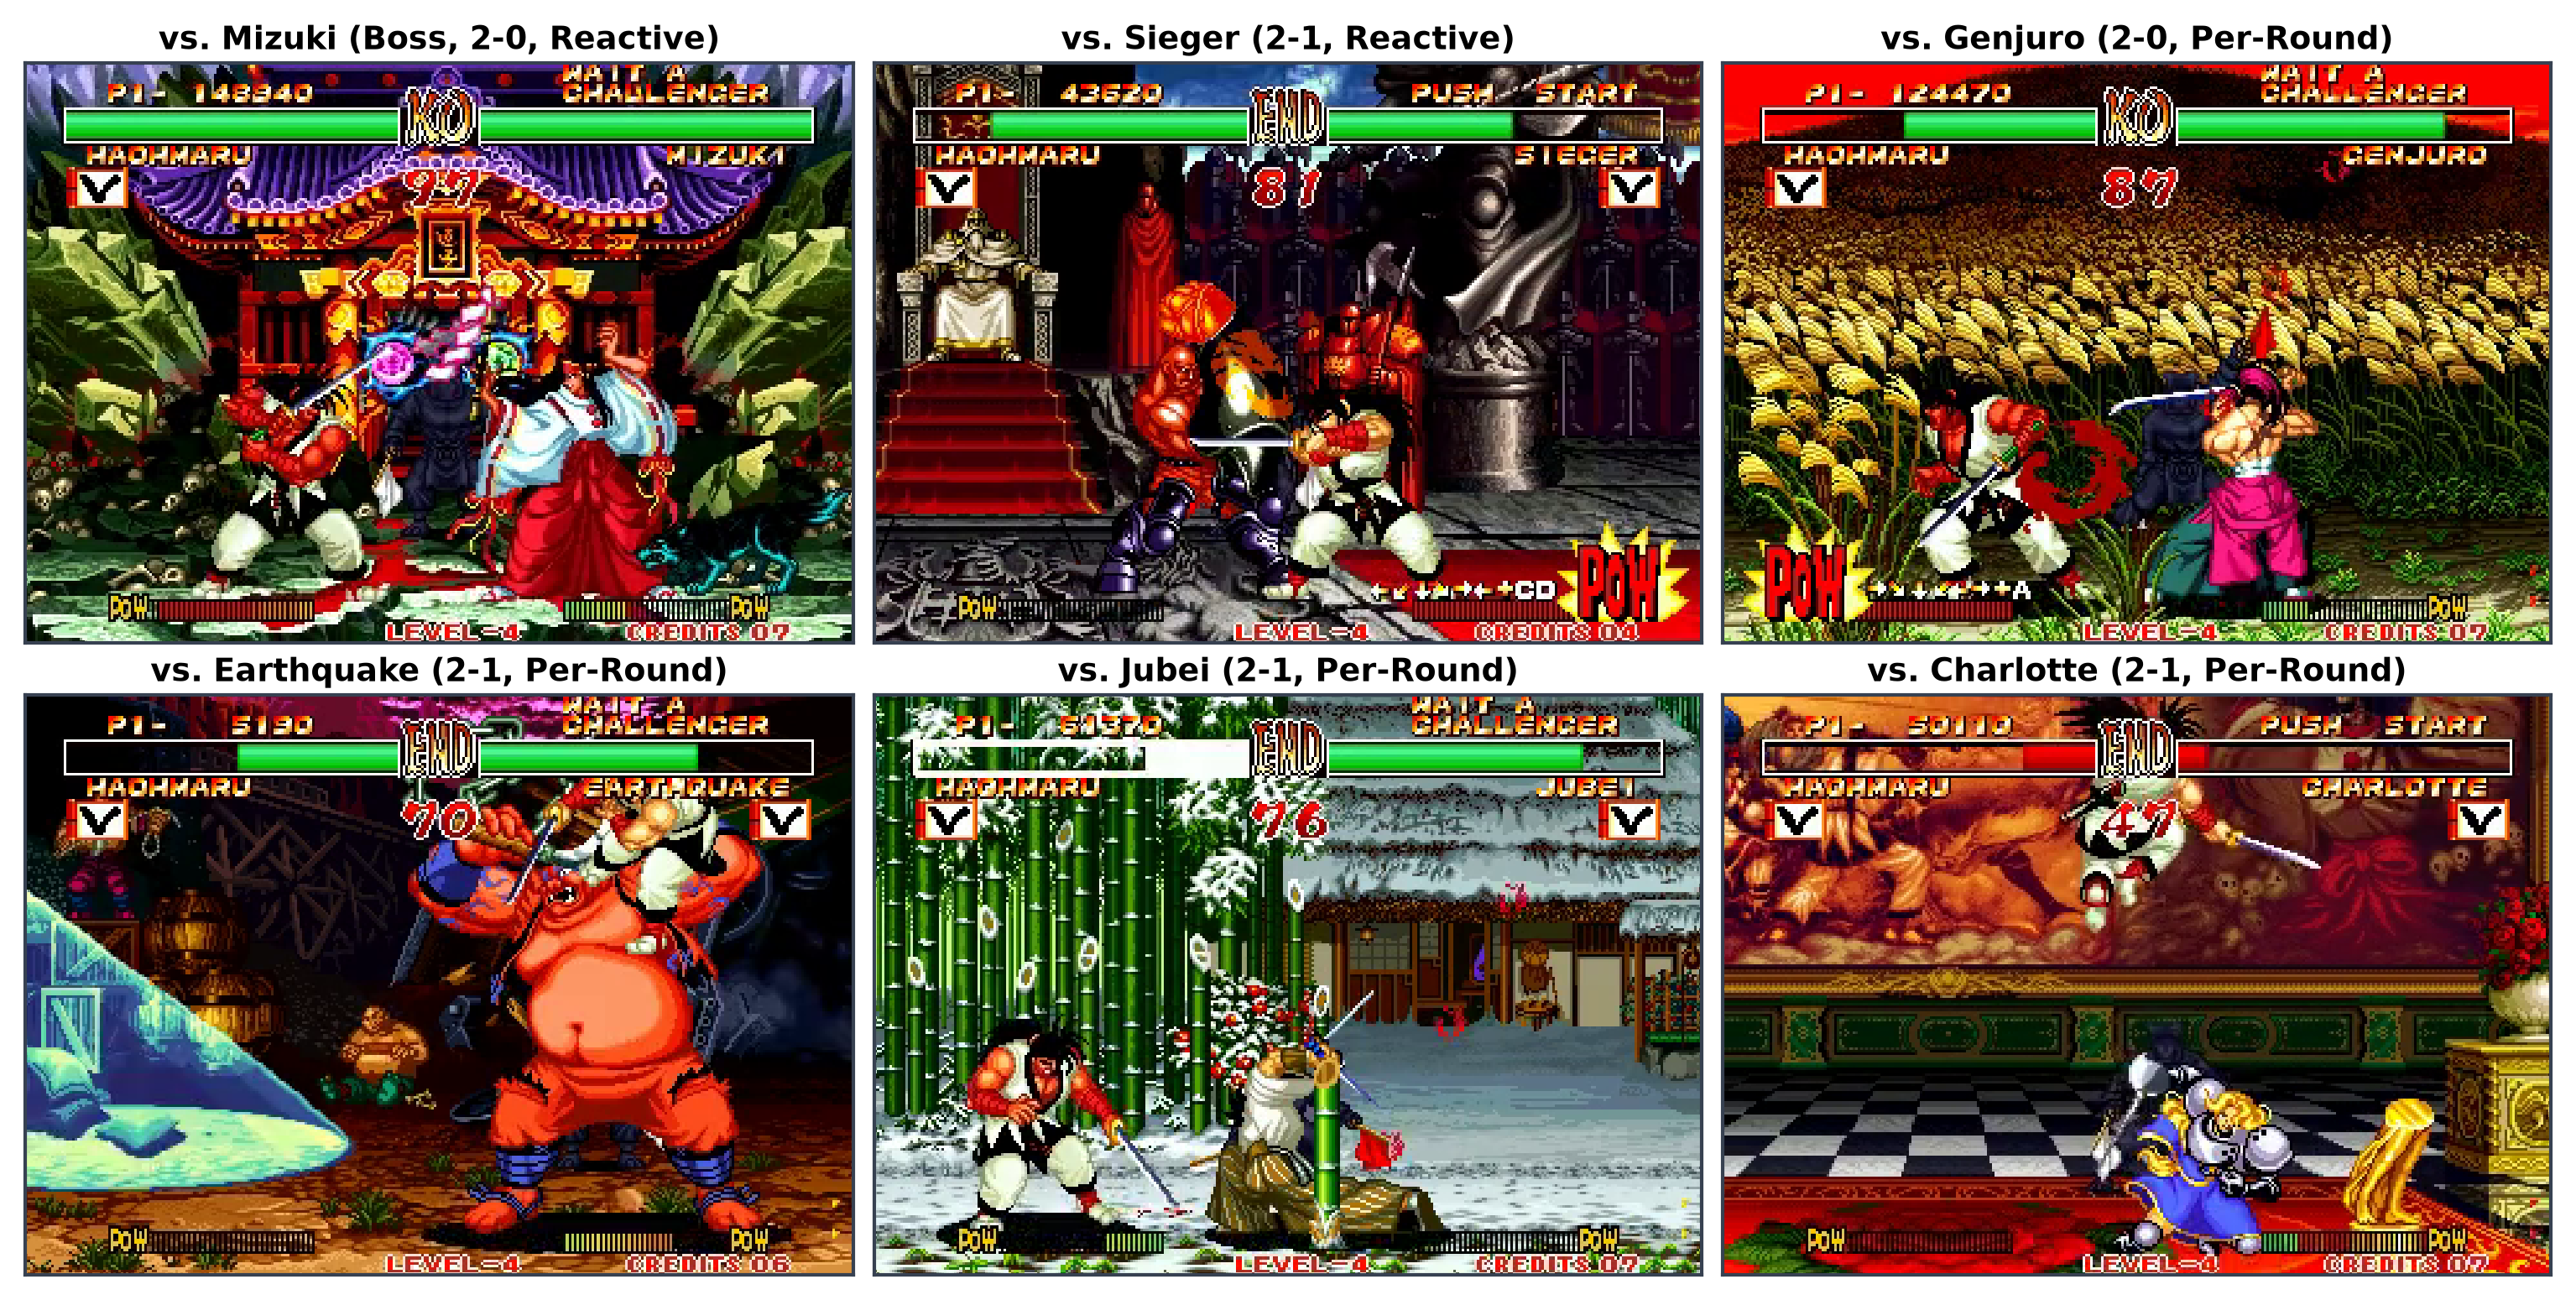
\includegraphics[width=0.96\textwidth]{figures/fig2_gameplay_montage.png}
    \caption{Representative live 60~FPS gameplay frames extracted from our verified Best-of-3 MP4 recordings across six matchups, including closed-loop distance-reactive victories over final boss Mizuki (2--0) and Sieger (2--1) and per-round expert wins over Genjuro, Earthquake, Jubei, and Charlotte.}
    \label{fig:montage}
\end{figure*}

\section{Experimental Evaluation \& Results}
\subsection{16/16 Full-Roster Bo3 Verification}
All 16 opponents were evaluated on live MAME 0.281 at native 1$\times$ speed (\texttt{--mode bo3 --speed 1}) using \texttt{tools/record\_match\_mp4.py}. Each match passed a physical quality gate audited via \texttt{ffprobe} and \texttt{\_commentary.json}: score strictly \texttt{2-0} or \texttt{2-1}, continuous duration $\ge 78$~s, an explicit 18.0-second post-KO celebration hold verifying authentic in-game victory banners, and synchronized Chinese/English SRT subtitles. Figure~\ref{fig:montage} shows six real frames extracted from these recordings, Figure~\ref{fig:perf} compares match durations and policy types across all 16 opponents, and Table~\ref{tab:results} lists the complete verified dataset.

\begin{figure}[t]
    \centering
    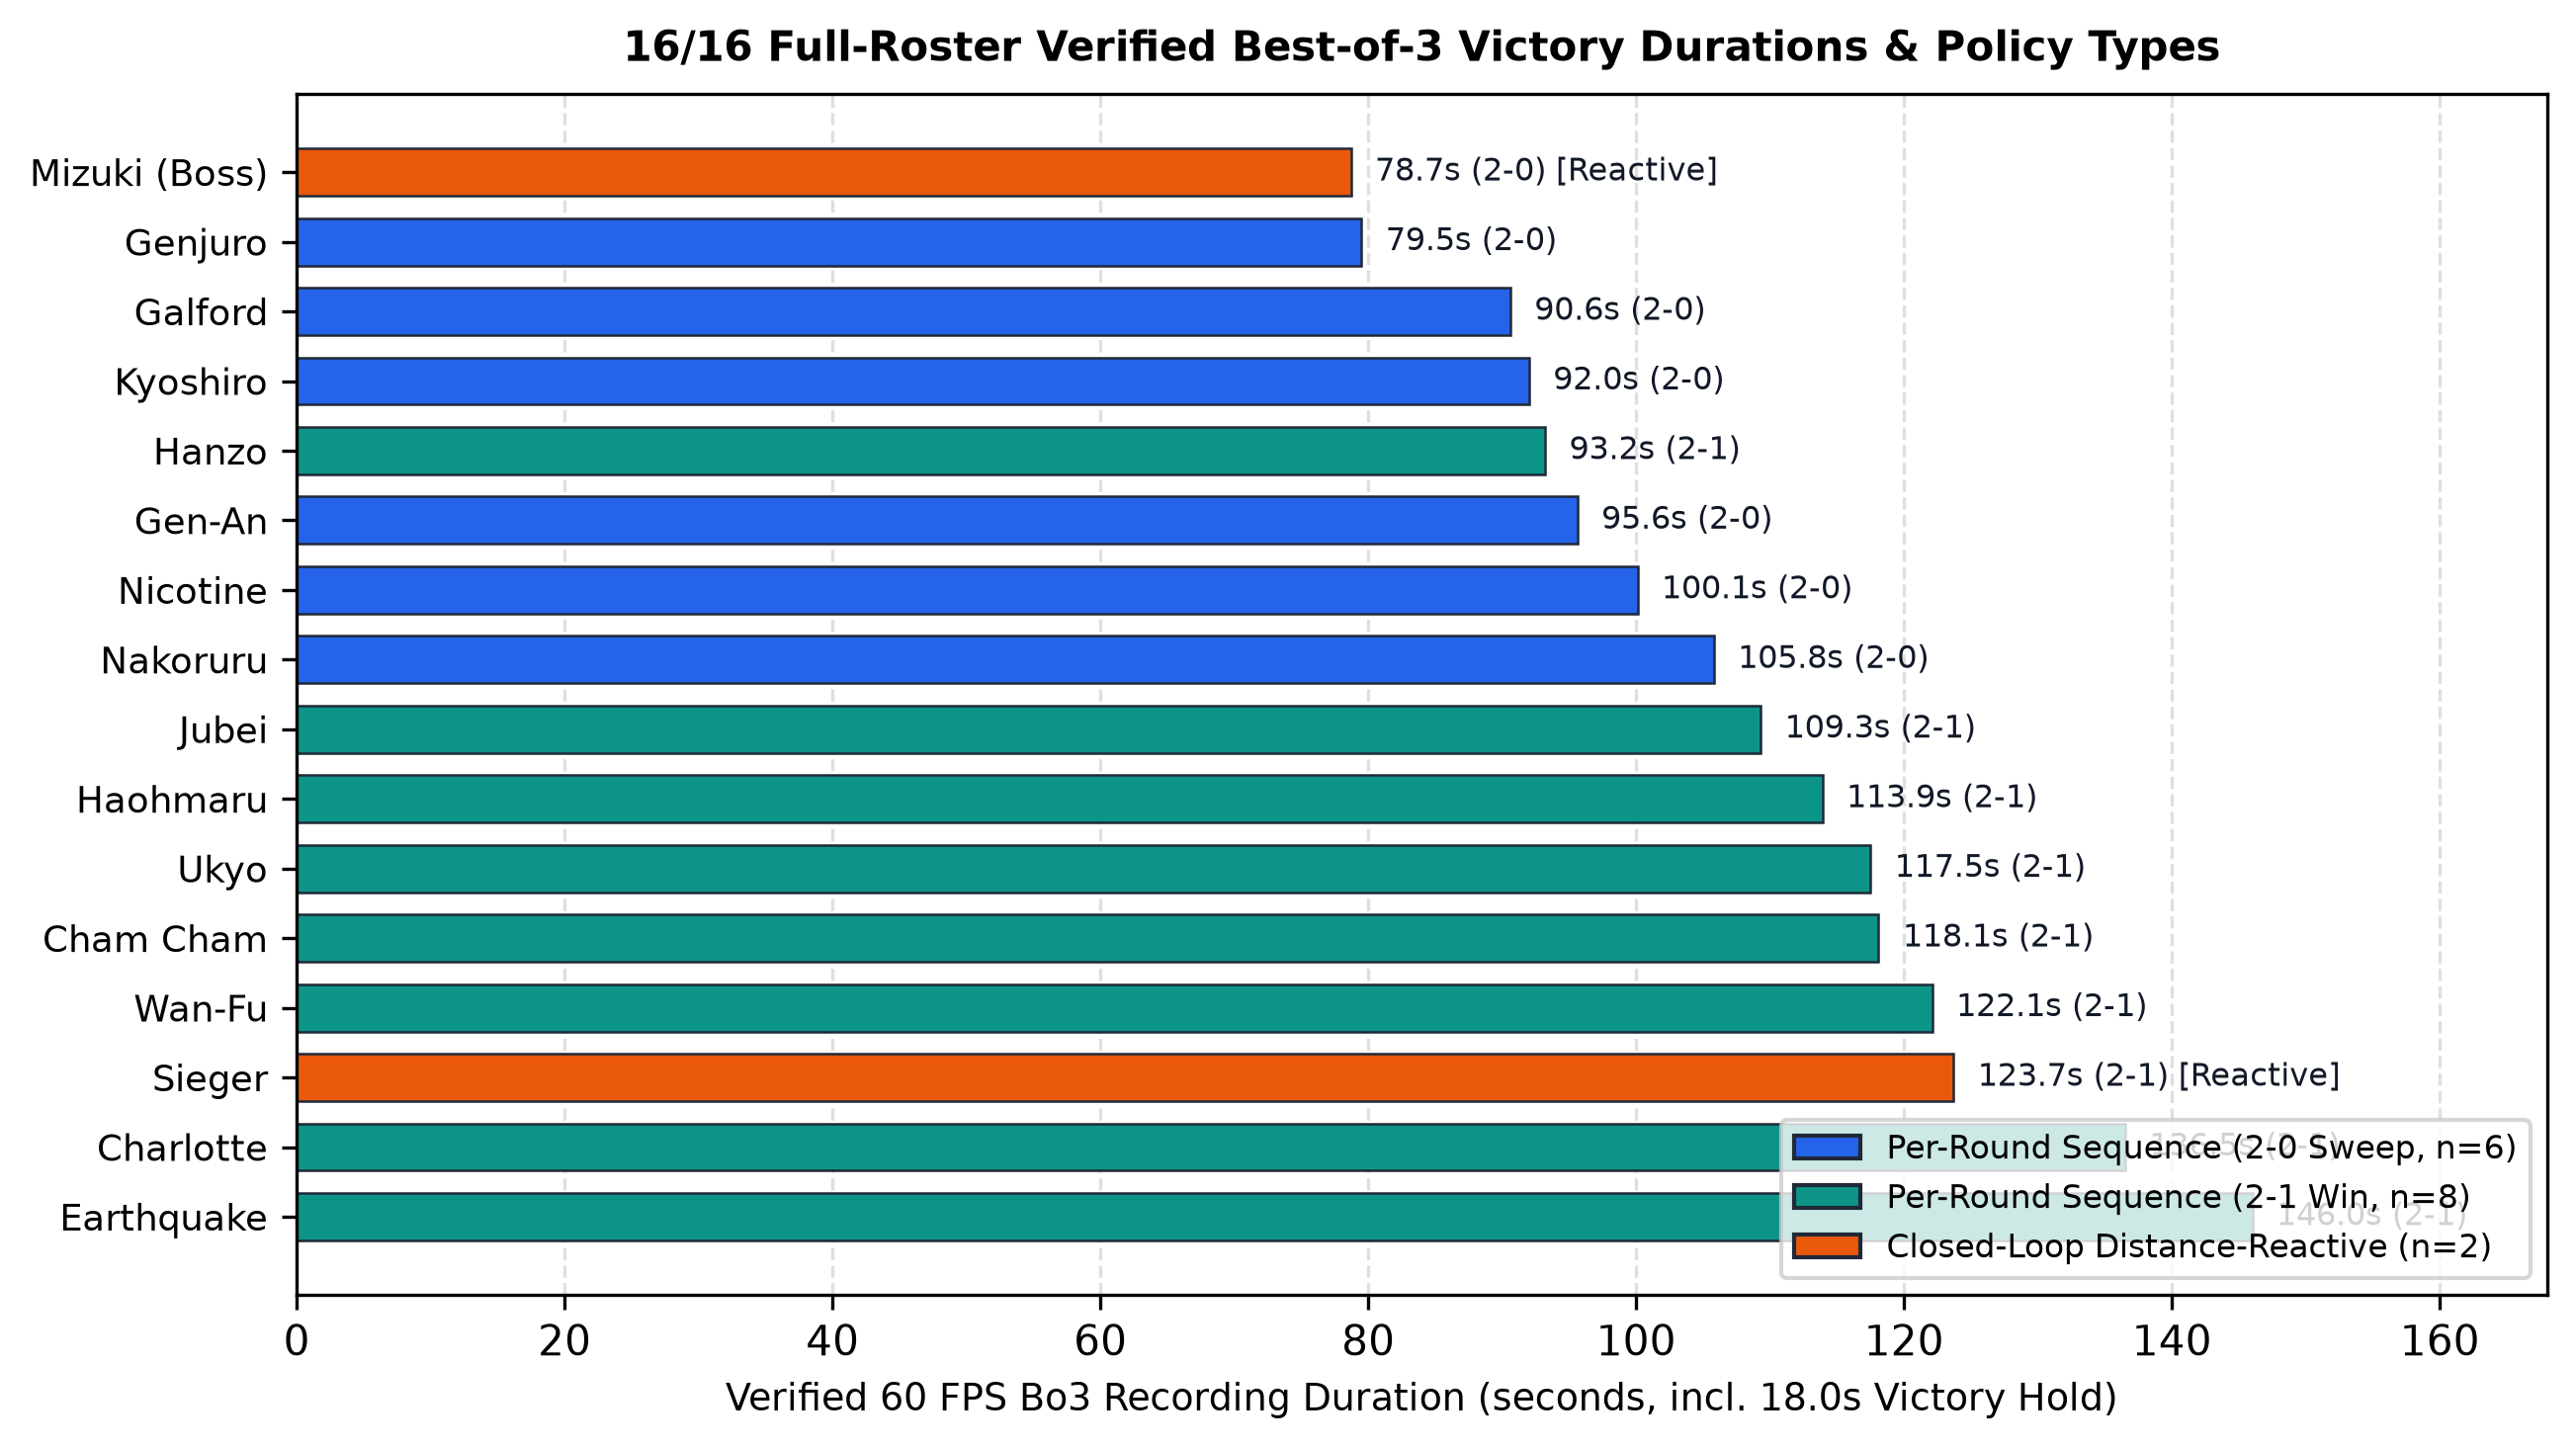
\includegraphics[width=\columnwidth]{figures/fig3_roster_performance.png}
    \caption{Verified 60~FPS Best-of-3 match durations (including 18.0~s post-KO victory hold), scores, and policy types across all 16 opponents.}
    \label{fig:perf}
\end{figure}

\begin{table}[t]
\centering
\caption{Complete 16/16 Verified Bo3 Results (Live 1$\times$ 60~FPS MAME)}
\label{tab:results}
\scriptsize
\begin{tabular}{r l c r r l}
\hline
\textbf{\#} & \textbf{Opponent} & \textbf{Score} & \textbf{Dur. (s)} & \textbf{MB} & \textbf{Policy Type} \\
\hline
1  & Earthquake      & 2--1 & 146.0 & 30.13 & Per-Round Seq \\
2  & Genjuro         & 2--0 &  79.5 & 20.15 & Per-Round Seq \\
3  & Galford         & 2--0 &  90.6 & 16.77 & Per-Round Seq \\
4  & Nakoruru        & 2--0 & 105.8 & 19.97 & Per-Round Seq \\
5  & Cham Cham       & 2--1 & 118.1 & 21.04 & Per-Round Seq \\
6  & Wan-Fu          & 2--1 & 122.1 & 26.46 & Per-Round Seq \\
7  & Sieger          & 2--1 & 123.7 & 19.50 & \textbf{Reactive} \\
8  & Kyoshiro        & 2--0 &  92.0 & 17.27 & Per-Round Seq \\
9  & Hanzo           & 2--1 &  93.2 & 13.55 & Per-Round Seq \\
10 & Gen-An          & 2--0 &  95.6 & 19.90 & Per-Round Seq \\
11 & Nicotine        & 2--0 & 100.1 & 15.69 & Per-Round Seq \\
12 & Mizuki (Boss)   & 2--0 &  78.7 & 19.23 & \textbf{Reactive} \\
13 & Haohmaru        & 2--1 & 113.9 & 20.78 & Per-Round Seq \\
14 & Ukyo            & 2--1 & 117.5 & 17.30 & Per-Round Seq \\
15 & Jubei           & 2--1 & 109.3 & 19.14 & Per-Round Seq \\
16 & Charlotte       & 2--1 & 136.5 & 22.94 & Per-Round Seq \\
\hline
\multicolumn{2}{l}{\textbf{Total / Mean}} & \textbf{16/16} & \textbf{107.7} & \textbf{19.95} & \textbf{14 Seq / 2 React} \\
\hline
\end{tabular}
\end{table}

Across all 16 matchups, AI Haohmaru achieved 7 clean 2--0 sweeps (43.8\%) and 9 hard-fought 2--1 victories (56.3\%), with a mean full-match recording length of 107.7~s (range 78.7--146.0~s).

\subsection{True 2P VS Human-vs-AI Verification}
To test real interactive play without input contention, we implemented True 2P VS mode (\texttt{.\textbackslash play\_demo.ps1 -Human}): MAME enables Freeplay (\texttt{DSW:64:1}) and injects 2P Start (\texttt{role=2, mask=0x04}) to trigger the authentic arcade \emph{"Here Comes a New Challenger"} character-select screen. All 1P keyboard bindings are disabled (\texttt{NONE}) while 2P is mapped to \texttt{WASD + J/K/L/U/I/O}. Upon match start, WRAM reads \texttt{UID + E\_CHAR} to route \texttt{MoEAgent} to the human's chosen fighter. Live human testing confirmed both strong offensive pressure from AI Haohmaru and exposed the two real-world defects (hardware ID offset \texttt{0x0B}--\texttt{0x10} and phantom R2 flicker) that we subsequently fixed and unit-tested.

\section{Limitations \& MoE-to-RL Roadmap}
We explicitly acknowledge two limitations of the current system:
\begin{enumerate}
    \item \textbf{Sequence Generalization Gap}: While the 14 sequence-based experts are highly reliable against deterministic arcade CPU state machines, human players can exploit fixed cadences via repeated low slides (observed empirically with human-controlled Cham Cham) or max-range whiff-baiting.
    \item \textbf{Lockstep Pacing}: Current human-vs-AI play steps 2 frames per bridge round-trip ($\approx 45$--60~FPS effective cadence) rather than fully asynchronous freeflow inference.
\end{enumerate}

Rather than treating MoE and deep RL as competing paradigms, our delivered 16/16 MoE library provides an ideal bootstrap for neural RL (detailed in our companion roadmap under \texttt{finaldoc/en/}):
\begin{itemize}
    \item \textbf{BC Cold-Start + Critic-Warmed PPO}: Replay all 16 experts inside \texttt{SS2RoundEnv} (with mild opening perturbation) to collect full 50-D \texttt{(obs, act, r, s', done)} trajectories, pretrain an SB3 policy via Behavior Cloning, freeze the actor while warming up the critic, and then fine-tune with low-LR PPO.
    \item \textbf{Kickstarting Distillation}~\cite{schmitt2018kickstarting}: Add a decaying $\lambda(t) D_{\text{KL}}(\pi_{\text{MoE}} \,\|\, \pi_{\text{PPO}})$ term to preserve defensive habits while allowing PPO to surpass the teacher on unseen states.
    \item \textbf{Go-Explore Endgames \& Offline RL}~\cite{ecoffet2021goexplore,kostrikov2022iql}: Save mid-round savestates from MoE rollouts for backplay curriculum learning, or combine MoE wins with exploratory PPO failures for pure-GPU IQL training.
\end{itemize}

\section{Conclusion}
We presented a practical, hardware-grounded Mixture-of-Experts architecture for \textit{Samurai Shodown II} that achieves 16/16 verified Best-of-3 victories on a single Windows machine. Beyond the 16/16 roster clear itself, our key engineering takeaways are that direct WRAM perception, semantic SMDP intent abstraction, closed-loop distance reactivity, and physical-invariant evaluation guards are decisive for building trustworthy fighting-game AI systems. The complete 92-file clean release, bilingual documentation, and verification tools are publicly available at \url{https://github.com/footballqq/samsho2-moe-ai}.

\begin{thebibliography}{9}
\bibitem{schulman2017ppo}
J.~Schulman, F.~Wolski, P.~Dhariwal, A.~Radford, and O.~Klimov, ``Proximal policy optimization algorithms,'' \textit{arXiv preprint arXiv:1707.06347}, 2017.

\bibitem{sutton1999options}
R.~S. Sutton, D.~Precup, and S.~Singh, ``Between MDPs and semi-MDPs: A framework for temporal abstraction in reinforcement learning,'' \textit{Artificial Intelligence}, vol.~112, no.~1--2, pp.~181--211, 1999.

\bibitem{jacobs1991moe}
R.~A. Jacobs, M.~I. Jordan, S.~J. Nowlan, and G.~E. Hinton, ``Adaptive mixtures of local experts,'' \textit{Neural Computation}, vol.~3, no.~1, pp.~79--87, 1991.

\bibitem{lu2013fightingice}
F.~Lu, K.~Yamamoto, L.~H. Nomura, S.~Mizuno, Y.~Lee, and R.~Thawonmas, ``Fighting game artificial intelligence competition platform,'' in \textit{Proc. IEEE Global Conf. on Consumer Electronics (GCCE)}, 2013, pp.~320--323.

\bibitem{vinyals2019alphastar}
O.~Vinyals \textit{et al.}, ``Grandmaster level in StarCraft II using multi-agent reinforcement learning,'' \textit{Nature}, vol.~575, pp.~350--354, 2019.

\bibitem{amodei2016concrete}
D.~Amodei \textit{et al.}, ``Concrete problems in AI safety,'' \textit{arXiv preprint arXiv:1606.06565}, 2016.

\bibitem{schmitt2018kickstarting}
S.~Schmitt \textit{et al.}, ``Kickstarting deep reinforcement learning,'' \textit{arXiv preprint arXiv:1803.03835}, 2018.

\bibitem{ecoffet2021goexplore}
A.~Ecoffet, J.~Huizinga, J.~Lehman, K.~O. Stanley, and J.~Clune, ``First return, then explore,'' \textit{Nature}, vol.~590, pp.~580--586, 2021.

\bibitem{kostrikov2022iql}
I.~Kostrikov, A.~Nair, and S.~Levine, ``Offline reinforcement learning with implicit Q-learning,'' in \textit{Proc. Int. Conf. on Learning Representations (ICLR)}, 2022.
\end{thebibliography}

\end{document}
